\chapter{图算法之最小生成树}

\begin{introduction}
	\item 问题概述
	\item Prim算法
	\item Kruskal算法
\end{introduction}

\section{概述}
给定一张边带权的无向图G=(V, E),其中V表示图中点的集合,E表示图中边的集合,n=|V|,m=|E|。
由V中的全部n个顶点和E中n-1条边构成的无向连通子图被称为G的一棵生成树,其中边的权值之和最小的生成树被称为无向图G的最小生成树。

最小生成树最为经典的两个算法分别是Prim算法和Kruskal算法。本节将首先讨论这两个算法的执行过程。

\section{基本概念}
在深入探讨之前,还需明白一些定义:

\begin{definition}{path}{path}
	A path is a sequence of edges which connects a sequence of nodes.
\end{definition}

\begin{definition}{cycle}{cycle}
	A cycle is a path with no repeated nodes or edges other than the
starting and ending nodes.
\end{definition}

可以借助\autoref{fig:path-cycle}理解path以及cycle的概念。

\begin{figure}[hbt]
	\centering
	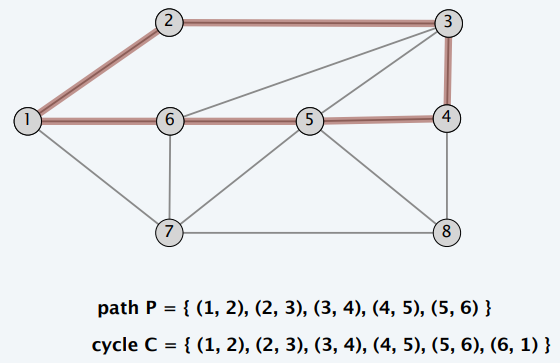
\includegraphics[scale=0.5]{image/pathcycle.png}
	\caption{具体例子说明path和cycle}\label{fig:path-cycle}
\end{figure}

\begin{definition}{cut}{MSTcut}
	A cut is a partition of the nodes into two nonempty subsets S and V / S.
\end{definition}

\begin{definition}{cutset}{MSTcutset}
	The cutset of a cut S is the set of edges with exactly one endpoint in S.
\end{definition}

可以借助\autoref{fig:cut-cutset}理解cut以及cutset的概念。

\begin{figure}[hbt]
	\centering
	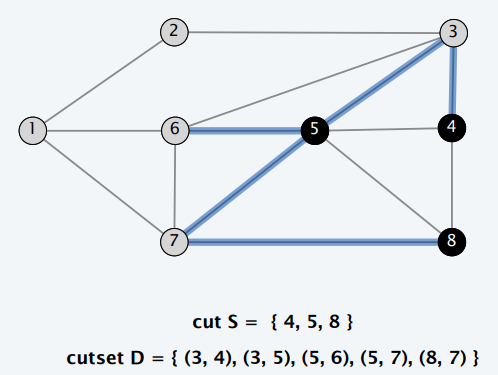
\includegraphics[scale=0.5]{image/cutcutset.png}
	\caption{具体例子说明cut与cutset}\label{fig:cut-cutset}
\end{figure}

\begin{theorem}{}{cycle-cutset-theorem}
	A cycle and a cutset intersect in an even number of edges.
\end{theorem}

可以借助\autoref{fig:cycle-cutset}理解\autoref{cycle-cutset-theorem}。

\begin{figure}[hbt]
	\centering
	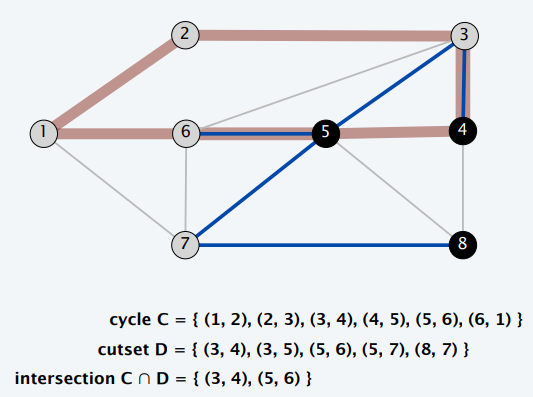
\includegraphics[scale=0.5]{image/cyclecutset.png}
	\caption{cycle、cutset的性质}\label{fig:cycle-cutset}
\end{figure}

\begin{definition}{生成树}{ST}
Let H = (V, T) be a subgraph of an undirected graph G = (V, E).
H is a spanning tree of G if H is both acyclic and connected.
\end{definition}

一个生成树的例子如\autoref{fig:exampleofST}所示。

\begin{figure}[hbt]
	\centering
	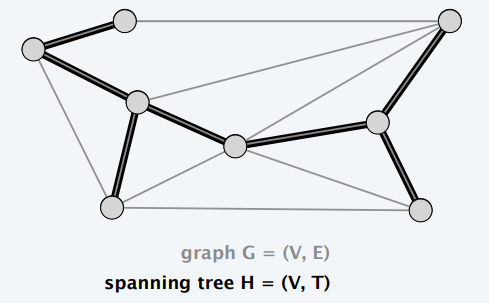
\includegraphics[scale=0.5]{image/exampleofST.png}
	\caption{生成树的例子}\label{fig:exampleofST}
\end{figure}

\begin{theorem}{}{ST-theorem}
	如果H = (V, T)是一个无向图G = (V, E)的子图,那么,以下各条件等价:
	\begin{enumerate}
		\item H是G的一棵生成树
		\item H是无环且连通的
		\item H是连通的并且有 V – 1条边
		\item H是无环的并且有 V – 1条边
		\item 任意拿掉H的一条边,就不再使其连通
		\item 任意增加一条边,则H就会构成环
	\end{enumerate}

\end{theorem}

\begin{definition}{最小生成树}{MST}
	Given a connected, undirected graph G = (V, E) with edge costs $c_e$,
a minimum spanning tree (V, T) is a spanning tree of G such that the sum
of the edge costs in T is minimized.
\end{definition}

一个生成树的例子如\autoref{fig:exampleofMST}所示。

\begin{figure}[hbt]
	\centering
	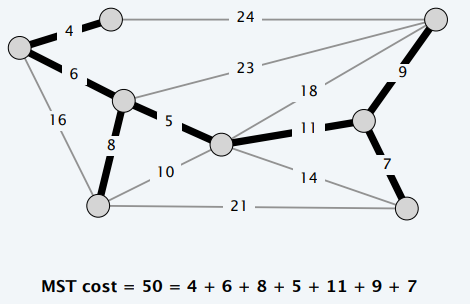
\includegraphics[scale=0.5]{image/exampleofMST.png}
	\caption{生成树的例子}\label{fig:exampleofMST}
\end{figure}

\begin{theorem}{Cayley’s theorem}{Cayley-theorem}
	The complete graph on n nodes has $n^(n–2)$ spanning trees
\end{theorem}

最小生成树是一个基础却有着十分广泛的应用的问题,之后的\autoref{sec:prim}和\autoref{sec:kruskal}
将分别介绍求解最小生成树的Prim算法和Kruskal算法。

\section{Prim算法}\label{sec:prim}
\subsection{算法描述与演示}
\begin{algorithm}
	\DontPrintSemicolon
	\KwIn{Graph G}
	\KwResult{MST of Graph G}
	\Begin{
		$S \leftarrow \{ s \} $ for any node s,$T \leftarrow \emptyset$;\\
		\For{$|T| < n-1$}{
			Add to T a min-weight edge with exactly one endpoint in S;\\
			Add the other endpoint to S;\\
		}
		Return T ;\\
	}
	\caption{Prim}\label{alg:Prim}
\end{algorithm}

算法执行流程如\autoref{fig:Prim}所示。

\begin{figure}[hbt]
	\centering
	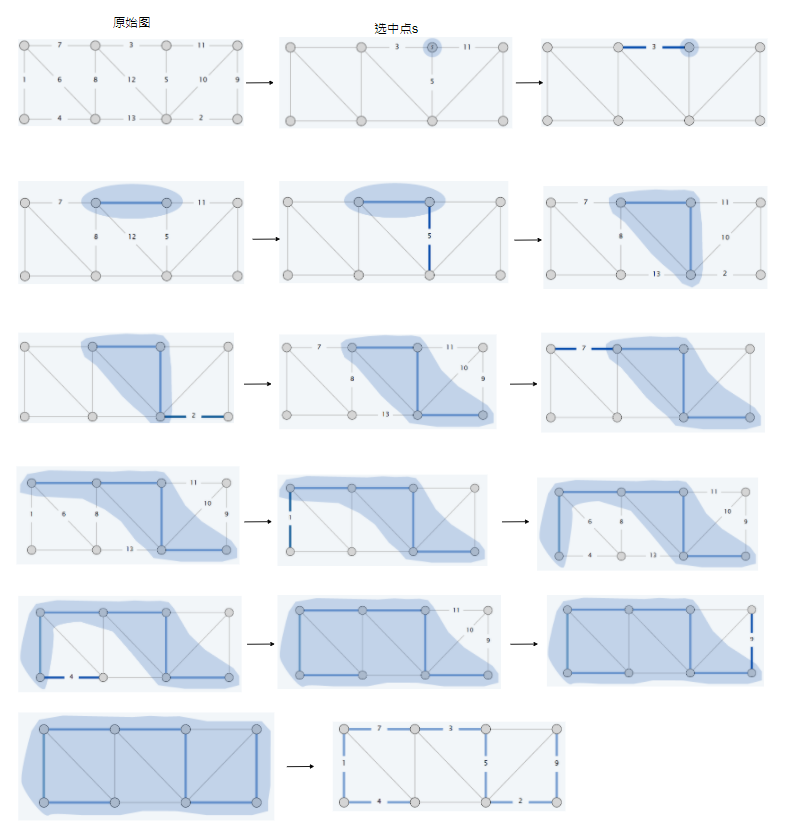
\includegraphics[scale=0.5]{image/prim.png}
	\caption{Prim算法的执行流程}\label{fig:Prim}
\end{figure}

\subsection{算法正确性证明}
记图G是一个连通图,Y是对p使用prim算法得到的一棵生成树,$Y_1$是p的一棵最小生成树
\begin{enumerate}
	\item 若Y=$Y_1$,显然prim算法是正确的
	\item 若Y≠$Y_1$,可进行如下推导:

	a)Y中有$n( n \geq 1 )$条边不存在于$Y_1$中,在构建Y的过程中,第一次遇到这样的一条边时(以e表示),
	则e的一个端点u落在V内(V是之前的prim运算得到的一个子顶点集),另一个端点v落在V外
	
	b)$Y_1$是连通的,故$Y_1$中存在u到v的一条的路径,此路径上必然存在一条边f,它的一个端点落在V内,另一个端点落在V外
	
	c)把e加入$Y_1$,去掉f,$Y_1$仍然连通,根据prim算法,权值$W(f) \geq W(e)$,否则e不会被选入V,
	如果$W(f)>W(e)$,新构建的树的权值和会比$Y_1$小,而$Y_1$是最小生成树,因此$W(f)>W(e)$不成立,得$W(f)=W(e)$
	
	d)对每一条类似e的边,重复过程c),最终Y和重新构建的的$Y_1$拥有的边完全一致,
	新构建的$Y_1$也是最小生成树,因此Y也是最小生成树,证明prim算法正确
\end{enumerate}

\subsection{算法复杂度}
普通堆优化的 Prim 算法复杂度为 $O(mlogn)$,而斐波那契堆优化的 Prim 算法
能达到 $O(m+nlogn)$

\section{Kruskal算法}\label{sec:kruskal}
\subsection{算法描述与演示}
\begin{algorithm}
	\DontPrintSemicolon
	\KwIn{Graph G}
	\KwResult{MST of Graph G}
	\Begin{
		$T \leftarrow \emptyset$;\\
		$S \leftarrow$sort edges by weight;\\
		\While{$e \in S$}{
			\If{$T \cup \{ e \}$ no cycle}{
				$T = T \cup \{ e \};$
			}
			\If{$|T| < n-1$}{
				Return T ;\\
			}
		}
	}
	\caption{kruskal}\label{alg:kruskal}
\end{algorithm}

算法执行流程如\autoref{fig:kruskal}所示。

\begin{figure}[hbt]
	\centering
	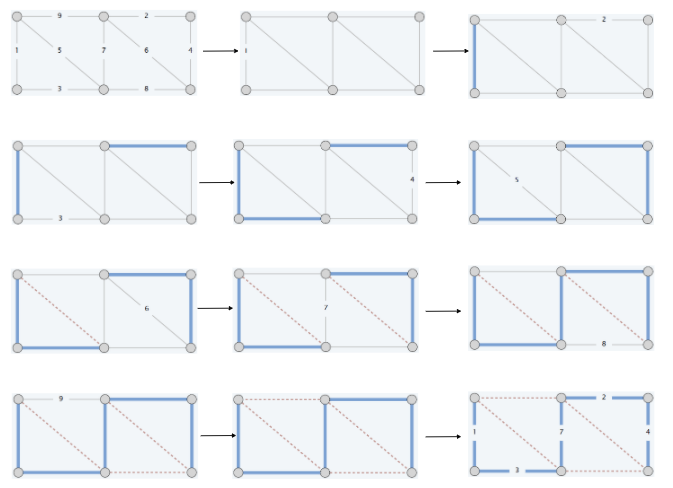
\includegraphics[scale=0.5]{image/kruskal.png}
	\caption{Kruskal算法的执行流程}\label{fig:kruskal}
\end{figure}

\subsection{算法正确性证明}
Kruskal算法每次会向T添加一条最小权重的边,并且不能形成环.
对于一棵树而言, 如果有K个节点, 则必然有K-1条边
我们要证明的问题其实是连续添加的边E(l) l=0,1,2...K-1 是一颗最小生成树MST的子集.

对于基本情况, 如果I = 0, 此时为空集,满足条件;

现在我们假设对 $0 \leq m < K-1$, E(m) 已经满足条件,是$T_1$的子集. 我们来看 E(m+1)的情况,
有E(m+1) = E(m) + {e}, e为算法当前新增的最小权重边.此时分两种情况:

\begin{enumerate}
	\item 如果{e}是$T_1$的子集,那么问题解决;
	\item 如果{e}不是$T_1$的子集, 那么我们要证明 E(m+1) 属于一颗其他的MST子集:

	因为{e}不是$T_1$的边, 所以 $T_1$ + {e} 必然有环C(性质1), 同时 E(m) 属于 $T_1$ ,
	那么在环C上必然有一个{e'} 不属于E(m) (因为如果属于E(m)的化, 那么算法当前选择的{e}会导致一个环, 与性质1违背).
	
	现在我们定义$T_2$ = $T_1$ + {e} - {e'}, 又因为E(m+1) = E(m) + {e} 所以 E(m+1) 属于$T_2$的子集.$T_2$是一颗MST.
	
	因为{e} 和 {e'} 都不属于 E(m), 算法当前选择的是{e} 说明 $weight({e'}) \geq weight({e})$.
	所以我们看$weight(T_2) = weight(T_1) + weight({e}) - weight({e'}) \leq weight(T_1)$ .
	
	这意味着$T_1$是$T_2$的权重upper-bound, 但由于$T_1$已经是MST, 所以必然的$T_2$也是MST. 至此得证.	
\end{enumerate}

\subsection{算法复杂度分析及优化}
\begin{theorem}{}{Kruskal-theorem}
	Kruskal’s algorithm can be implemented to run in $O(m log m)$ time.
\end{theorem}

\begin{enumerate}
	\item Sort edges by cost:$O(m log m)$.
	\item Use union–find data structure to dynamically maintain connected components:$O(m \alpha (n))$.
\end{enumerate}

\begin{remark}
	$\alpha (n)$是反阿克曼函数,阿克曼函数 $A(m,n)$ 增长极快,其反函数几乎是常数。
\end{remark}

下面将简要介绍并查集(union–find data structure)有关内容。
\subsection{并查集}
在计算机科学中,并查集是一种树型的数据结构,用于处理一些不交集(Disjoint Sets)的合并及查询问题。
有一个联合-查找算法(union-find algorithm)定义了两个用于此数据结构的操作:

Find:确定元素属于哪一个子集。它可以被用来确定两个元素是否属于同一子集。

Union:将两个子集合并成同一个集合。

在并查集森林中,每个集合的代表即是集合的根节点。“查找”根据其父节点的引用向根行进直到到底树根。
“联合”将两棵树合并到一起,这通过将一棵树的根连接到另一棵树的根。实现这样操作的一种方法是

\begin{lstlisting}
function MakeSet(x)
     x.parent := x

function Find(x)
     if x.parent == x
        return x
     else
        return Find(x.parent)

function Union(x, y)
     xRoot := Find(x)
     yRoot := Find(y)
     xRoot.parent := yRoot
\end{lstlisting}

这是并查集森林的最基础的表示方法,这个方法不会比链表法好,这是因为创建的树可能会严重不平衡;然而,可以用两种办法优化。

第一种方法,称为“按秩合并”,即总是将更小的树连接至更大的树上。因为影响运行时间的是树的深度,
更小的树添加到更深的树的根上将不会增加秩除非它们的秩相同。在这个算法中,术语“秩”替代了“深度”,因为同时应用了路径压缩时秩将不会与高度相同。

第二个优化,称为“路径压缩”,是一种在执行“查找”时扁平化树结构的方法。关键在于在路径上的每个节点都可以直接连接到根上;
他们都有同样的表示方法。为了达到这样的效果,Find递归地经过树,改变每一个节点的引用到根节点。得到的树将更加扁平。
